% Standalone TikZ figure: Framework Selection Decision Tree
% For Chapter 4: Synthetic Data Generation for Object Detection
\documentclass[tikz,border=10pt]{standalone}
\usepackage{tikz}
\usetikzlibrary{arrows.meta, positioning, shapes.geometric, fit, backgrounds, calc}

\begin{document}
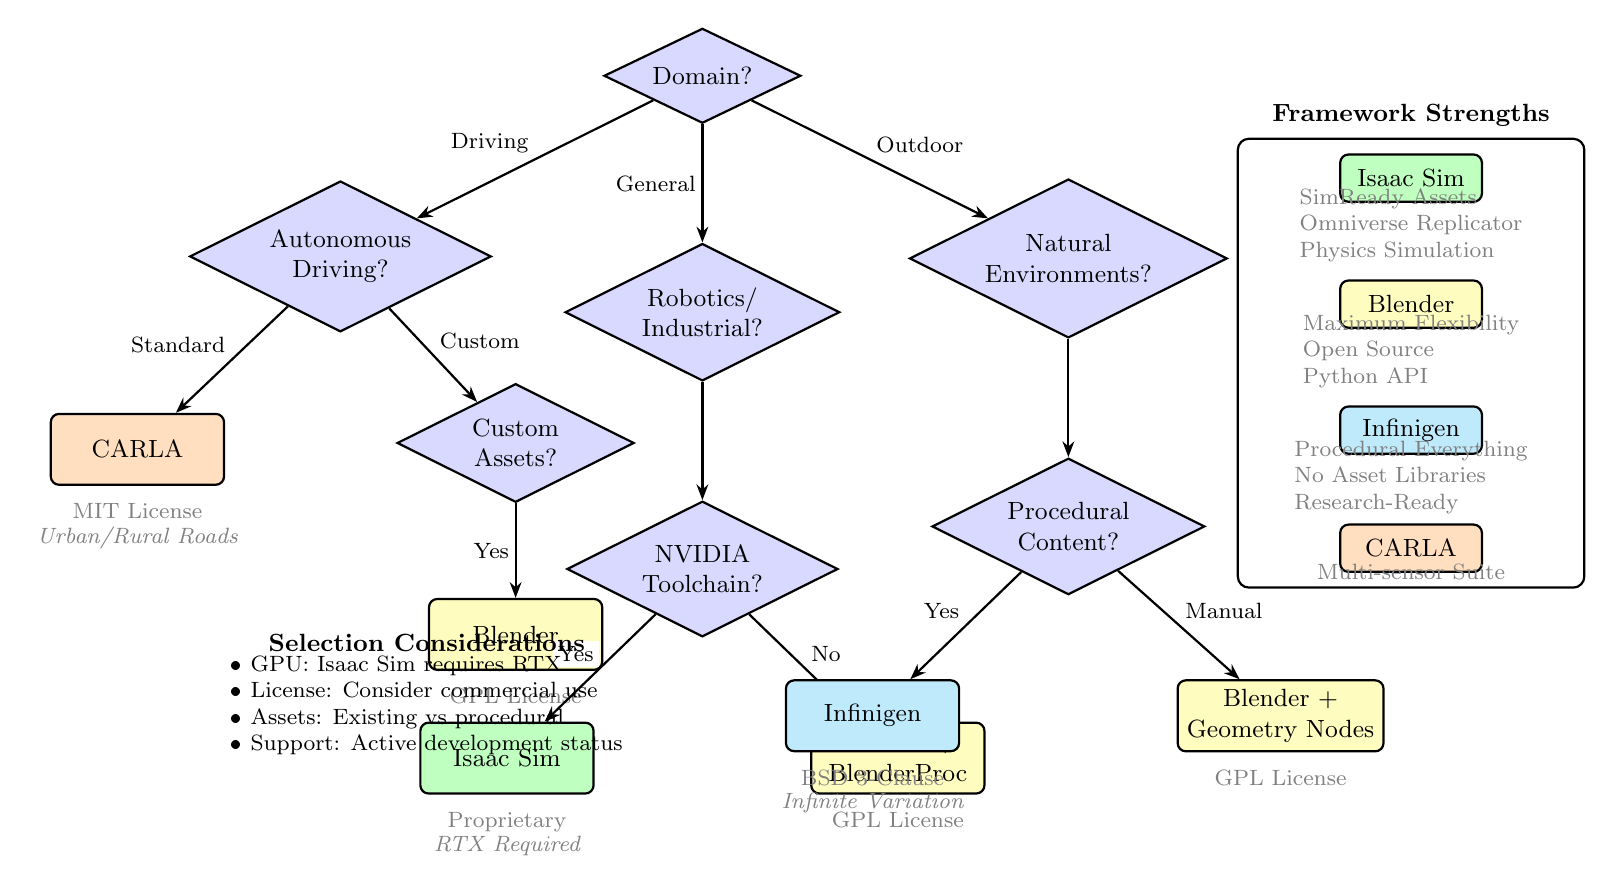
\begin{tikzpicture}[
    every node/.style={font=\small},
    decision/.style={diamond, draw, thick, aspect=2, minimum width=2.5cm, minimum height=1.2cm, align=center, fill=blue!15},
    framework/.style={rectangle, draw, thick, minimum width=2.2cm, minimum height=0.9cm, align=center, rounded corners=3pt},
    arrow/.style={-{Stealth[length=2mm]}, thick},
    yesno/.style={font=\footnotesize, fill=white, inner sep=2pt}
]

% Root decision
\node[decision] (start) at (0, 0) {Domain?};

% Level 1 branches
\node[decision, below left=1.5cm and 3cm of start] (auto) {Autonomous\\Driving?};
\node[decision, below=1.5cm of start] (robot) {Robotics/\\Industrial?};
\node[decision, below right=1.5cm and 3cm of start] (env) {Natural\\Environments?};

% Arrows from root
\draw[arrow] (start) -- node[yesno, above left] {Driving} (auto);
\draw[arrow] (start) -- node[yesno, left] {General} (robot);
\draw[arrow] (start) -- node[yesno, above right] {Outdoor} (env);

% CARLA branch
\node[framework, fill=orange!25, below left=1.5cm and 0.5cm of auto] (carla) {CARLA};
\node[font=\footnotesize, text=gray, below=0.1cm of carla] {MIT License};
\node[font=\footnotesize\itshape, text=gray, below=0.4cm of carla] {Urban/Rural Roads};

% Blender branch for driving alternative
\node[decision, below right=1.5cm and 0.5cm of auto] (custom) {Custom\\Assets?};

% Arrows from auto
\draw[arrow] (auto) -- node[yesno, above left] {Standard} (carla);
\draw[arrow] (auto) -- node[yesno, above right] {Custom} (custom);

% From custom driving
\node[framework, fill=yellow!25, below=1.2cm of custom] (blender1) {Blender};
\node[font=\footnotesize, text=gray, below=0.1cm of blender1] {GPL License};

\draw[arrow] (custom) -- node[yesno, left] {Yes} (blender1);

% Robotics branch
\node[decision, below=1.5cm of robot] (nvidia) {NVIDIA\\Toolchain?};

% Isaac Sim
\node[framework, fill=green!25, below left=1.5cm and 0.5cm of nvidia] (isaac) {Isaac Sim};
\node[font=\footnotesize, text=gray, below=0.1cm of isaac] {Proprietary};
\node[font=\footnotesize\itshape, text=gray, below=0.4cm of isaac] {RTX Required};

% Blender for robotics
\node[framework, fill=yellow!25, below right=1.5cm and 0.5cm of nvidia] (blender2) {Blender +\\BlenderProc};
\node[font=\footnotesize, text=gray, below=0.1cm of blender2] {GPL License};

% Arrows from nvidia
\draw[arrow] (robot) -- (nvidia);
\draw[arrow] (nvidia) -- node[yesno, above left] {Yes} (isaac);
\draw[arrow] (nvidia) -- node[yesno, above right] {No} (blender2);

% Environment branch
\node[decision, below=1.5cm of env] (proc) {Procedural\\Content?};

% Infinigen
\node[framework, fill=cyan!25, below left=1.5cm and 0.5cm of proc] (infinigen) {Infinigen};
\node[font=\footnotesize, text=gray, below=0.1cm of infinigen] {BSD 3-Clause};
\node[font=\footnotesize\itshape, text=gray, below=0.4cm of infinigen] {Infinite Variation};

% Blender for environments
\node[framework, fill=yellow!25, below right=1.5cm and 0.5cm of proc] (blender3) {Blender +\\Geometry Nodes};
\node[font=\footnotesize, text=gray, below=0.1cm of blender3] {GPL License};

% Arrows from proc
\draw[arrow] (env) -- (proc);
\draw[arrow] (proc) -- node[yesno, above left] {Yes} (infinigen);
\draw[arrow] (proc) -- node[yesno, above right] {Manual} (blender3);

% ============ KEY FEATURES BOX ============
\begin{scope}[shift={(9, -2)}]
    \node[font=\bfseries\small] at (0, 1.5) {Framework Strengths};

    \draw[thick, rounded corners] (-2.2, 1.2) rectangle (2.2, -4.5);

    \node[framework, fill=green!25, minimum width=1.8cm, minimum height=0.6cm] at (0, 0.7) {Isaac Sim};
    \node[font=\footnotesize, text=gray, align=left] at (0, 0.1) {SimReady Assets\\Omniverse Replicator\\Physics Simulation};

    \node[framework, fill=yellow!25, minimum width=1.8cm, minimum height=0.6cm] at (0, -0.9) {Blender};
    \node[font=\footnotesize, text=gray, align=left] at (0, -1.5) {Maximum Flexibility\\Open Source\\Python API};

    \node[framework, fill=cyan!25, minimum width=1.8cm, minimum height=0.6cm] at (0, -2.5) {Infinigen};
    \node[font=\footnotesize, text=gray, align=left] at (0, -3.1) {Procedural Everything\\No Asset Libraries\\Research-Ready};

    \node[framework, fill=orange!25, minimum width=1.8cm, minimum height=0.6cm] at (0, -4.0) {CARLA};
    \node[font=\footnotesize, text=gray, align=left] at (0, -4.3) {Multi-sensor Suite};
\end{scope}

% ============ CONSIDERATIONS ============
\begin{scope}[shift={(-5.5, -7.5)}]
    \node[font=\bfseries\small] at (2, 0.3) {Selection Considerations};

    \node[font=\footnotesize, align=left] at (2, -0.5) {
        \textbullet\ GPU: Isaac Sim requires RTX\\
        \textbullet\ License: Consider commercial use\\
        \textbullet\ Assets: Existing vs procedural\\
        \textbullet\ Support: Active development status
    };
\end{scope}

\end{tikzpicture}
\end{document}
